\chapter{Experiments \& Results}
\label{chap:impl}

This chapter presents a comprehensive examination of various experiments designed to investigate the effectiveness of knowledge distillation techniques in enhancing the performance of smaller models through the utilization of LLM\@. 

The experiments are systematically structured to compare baseline models, explore innovative architectural modifications, and assess the impact of training strategies on model accuracy and efficiency in sequence classification tasks. The experimental findings are crucial for validating the theoretical propositions discussed in previous chapters and for demonstrating the practical capabilities of distillation methodologies in real-world applications.

Additionally, this chapter aim to deepen the understanding of knowledge distillation processes and their practical applications in enhancing the efficacy of smaller models by leveraging the knowledge embedded within LLM\@. The results from these experiments will provide valuable insights that could reshape approaches to model training and optimization in the field of NLP\@.

\newcounter{experiment}
\stepcounter{experiment}
\section{Experiment \theexperiment: Evaluating the baselines}

In this section, I detail the methodologies and results of the experiment aimed at evaluating the baseline models described in \autoref{sec:baselines}. The primary goal of this experiment is to assess the performance of each model across datasets provided in \autoref{sec:datasets} to establish a benchmark for future comparative analyses.

Prior to the training process, the datasets were segmented into smaller portions (\autoref{tab:dataset_portions}). The rationale behind selecting varied dataset sizes, including smaller subsets and relatively larger subsets, is to enable a more precise evaluation of model distillation techniques across different scales of data. This approach allows for a detailed comparison of how data volume impacts the effectiveness of distillation in transferring knowledge from larger to smaller models. This standardized approach is crucial for mitigating variability in dataset size, which can influence the accuracy and reliability of the results, particularly when assessing model performance under different data constraints.

\begin{table}[h]
    \centering
    \caption{Number of samples in each dataset portion}
    \label{tab:dataset_portions}
    \resizebox{\textwidth}{!}{
        \begin{tabular}{lccccccccc}
            \toprule
                                         & \multicolumn{9}{c}{\textbf{Portion size}}                                                                                                                            \\
            \textbf{Dataset}             & \textbf{0.01}                             & \textbf{0.03} & \textbf{0.05} & \textbf{0.07} & \textbf{0.1} & \textbf{0.3} & \textbf{0.5} & \textbf{0.7} & \textbf{1.0} \\

            \midrule
            WOS (\autoref{sec:wos})      & N/A                                       & N/A           & N/A           & N/A           & 380          & 1,138        & 1,896        & 2,654        & 3,791        \\
            e-SNLI (\autoref{sec:esnli}) & 386                                       & 1,156         & 1,926         & 2,697         & 3,852        & 11,556       & 19,260       & 26,964       & 38,520       \\
            \bottomrule
        \end{tabular}
    }
\end{table}

Each model was trained on the datasets using a predefined split of training and validation data, same for each model. Model validation was performed intermittently during training to monitor performance, adjust parameters as necessary and use early stopping to prevent overfitting.

After training, each model was evaluated on a separate test set that was not used during the training or validation phases. This approach ensures that the performance metrics reflect the generalizability of each model.

The results of this experiment are presented in the Fig. \ref{fig:baselines:wos} and \ref{fig:baselines:esnli}, where the F1 score is utilized as the primary metric for model evaluation. The F1 score, a harmonized measure that incorporates precision, recall, and accuracy, is particularly effective in providing a balanced assessment of model performance.

\begin{figure}[p]
    \centering
    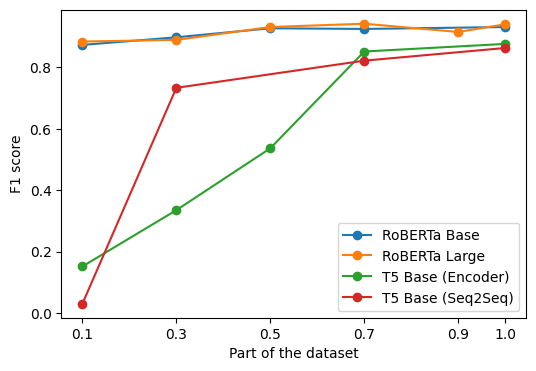
\includegraphics[width=0.6\linewidth]{figs/wos_baseline.png}
    \caption{F1 score performance of baseline models on the WOS dataset across varying dataset sizes.}
    \label{fig:baselines:wos}
\end{figure}
\begin{figure}[p]
    \centering
    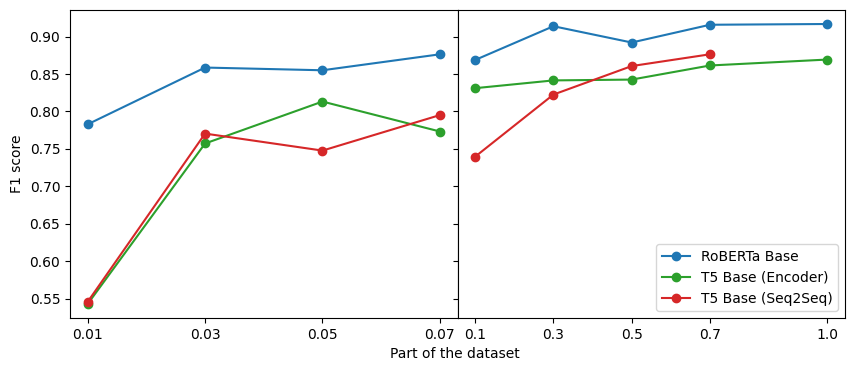
\includegraphics[width=\linewidth]{figs/esnli_baseline.png}
    \caption{F1 score performance of baseline models on the e-SNLI dataset across varying dataset sizes.}
    \label{fig:baselines:esnli}
\end{figure}

These figures vividly illustrate the performance of each model across various dataset sizes, offering a detailed visualization of the models' accuracy and efficiency.

This comprehensive overview allows for a nuanced analysis of how model effectiveness varies with the size of the dataset. RoBERTa models consistently outperformed T5 models, regardless of their setup, across all dataset sizes, demonstrating their superior performance in sequence classification tasks.

Additionally, RoBERTa exhibited less variance across different dataset sizes, indicating more robust and reliable performance. Conversely, the EncT5 model showed little improvement over the T5 Seq2Seq model, suggesting that the architectural modifications did not significantly enhance its classification capabilities.

These insights give rise to the hypothesis that models designed explicitly for classification, like RoBERTa, may be inherently more suitable for student model compared to more generative models like T5.

\newpage

\stepcounter{experiment}
\section{Experiment \theexperiment: Train T5 model with 2 heads}

The student model in this experiment employs a modified T5 architecture \cite{t5}, incorporating a dual-head design to enhance its functionality. This adaptation includes the addition of a classification head alongside the existing language modeling head, which is now specifically tasked with generating rationales (\autoref{fig:modified_t5}). The model is trained on a dataset that consists of labeled examples, with its training trajectory significantly informed by the LLM knowledge. But during the prediction phase, the classification head is used to make predictions, while the language modeling head is not utilized.

\begin{figure}[hbt]
    \centering
    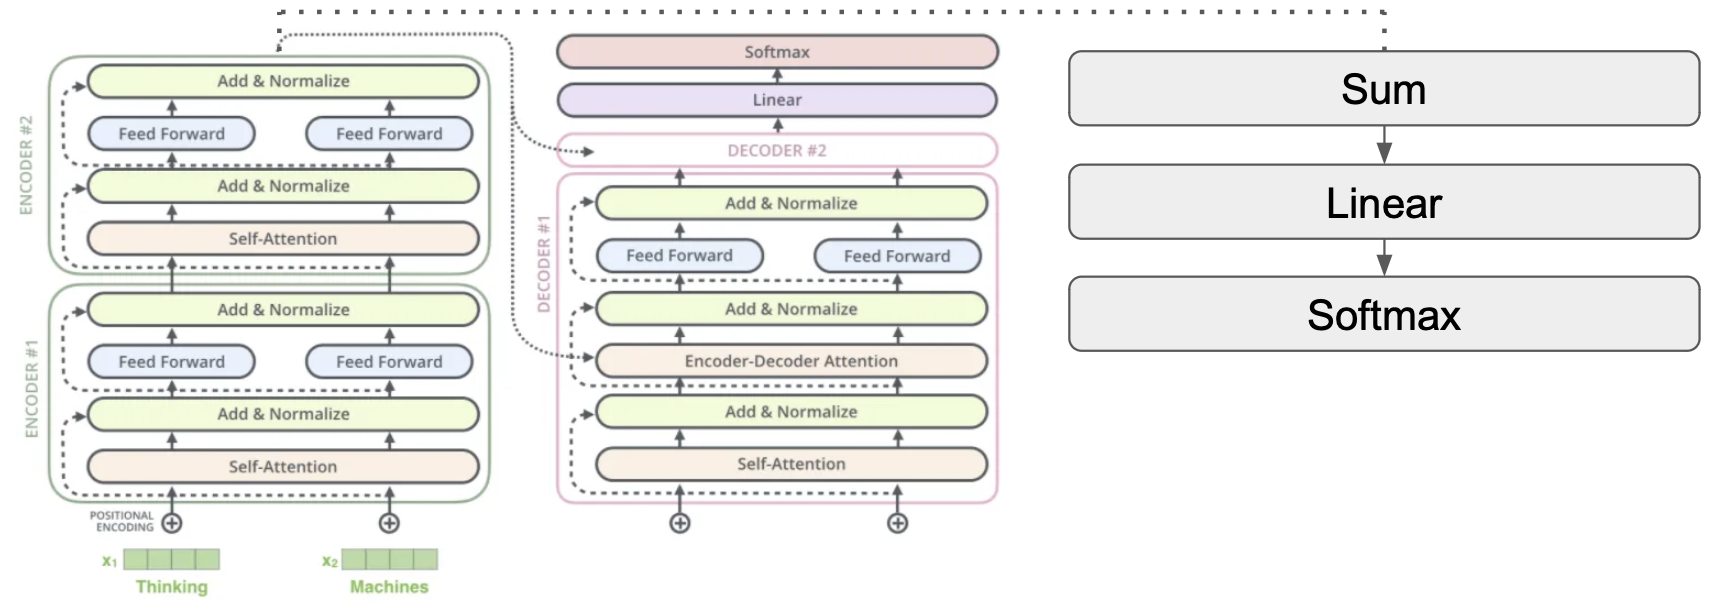
\includegraphics[width=0.99\linewidth]{figs/modified_t5.png}
    \caption{Modified T5 architecture for the student model.}
    \label{fig:modified_t5}
\end{figure}

The use of a linear combination for the loss function optimally balances the contributions from both language modeling and classification tasks during training. Specifically, the combined loss function can be formulated as follows
$$ L = \alpha L_{LM} + (1 - \alpha) L_{C} $$
Where $L$ represents the total loss, $L_{LM}$ is the original T5 language modeling loss, $L_{C}$ is the classification loss (cross-entropy), and $\alpha$ is a hyperparameter that determines the relative importance of the two losses.

Irrespective of the selected value for the parameter $\alpha$, there was no observed reduction in the classification loss. Language modeling loss, exhibited some decrease depends on $\alpha$, indicating that the model was learning to generate rationales. This phenomenon may be attributed to the possibility that the features extracted by the T5 encoder, which are utilized by the decoder, are insufficient for the classification task.

\ldots
